\documentclass[utf8]{psta}

\subjclass[UDC]{004.42}
\subjclass[BBC]{32.973}
\subjclass[2010]{68N19}

\title[векторизация римановского решателя]{Векторизация римановского решателя с использованием набора инструкций AVX-512}    

\author{Рыбаков, Алексей Анатольевич}
\address{Межведомственный суперкомпьютерный центр Российской академии наук -- филиал Федерального государственного учреждения <<Федеральный научный центр Научно-исследовательский институт системных исследований Российской академии наук>> (МСЦ РАН -- филиал ФГУ ФНЦ НИИСИ РАН), 119334, Москва, Ленинский проспект, 32а.}
\email{rybakov@jscc.ru}
%\thanks{TODO}
\info{Рыбаков Алексей Анатольевич -- к ф.-м. н., внс МСЦ РАН -- филиала ФГУ ФНЦ НИИСИ РАН. Области научных интересов -- математическое моделирование задач газовой динамики с использованием суперкомпьютеров, методы построения и управления расчетными сетками, дискретная математика, теория графов, модели случайных графов, параллельное программирование, функциональное программирование.}
\image{pics/rybakov}
\orcid{0000-0002-9755-8830}    

\author{Шумилин, Сергей Сергеевич}
\address{Межведомственный суперкомпьютерный центр Российской академии наук - филиал Федерального государственного учреждения <<Федеральный научный центр Научно-исследовательский институт системных исследований Российской академии наук>> (МСЦ РАН -- филиал ФГУ ФНЦ НИИСИ РАН), 119334, Москва, Ленинский проспект, 32а.}
\email{shumilin@jscc.ru}
%\thanks{TODO}
\info{Шумилин Сергей Сергеевич -- ведущий инженер МСЦ РАН -- филиала ФГУ ФНЦ НИИСИ РАН. Области научных интересов -- машинное обучение, анализ данных, алгоритмы, параллельное программирование.}
\image{pics/shumilin}
%\image{nobody}
\orcid{0000-0002-3953-7054}    

\keywords{задача Римана о распаде произвольного разрыва, римановский решатель, AVX-512, KNL, векторизация, функции-интринсики}
\begin{abstract}
Численные методы, базирующиеся на решении задачи Римана о распаде произвольного разрыва, крайне требовательны к вычислительным ресурсам.
Для применения данных численных методов на современных расчетных сетках требуется использование суперкомпьютера.
Среди различных инструментов повышения производительности суперкомпьютерных приложений можно выделить векторизацию программного кода.
Набор инструкций AVX-512 обладает рядом уникальных возможностей, позволяющих применить векторизацию к программному контексту римановского решателя, что ведет к значительному ускорению решателя.
На примере точного римановского решателя рассматривается практический подход к векторизации разнообразного программного контекста, включая простые линейные участки, регионы со сложным управлением, а также вложенные циклы.
В основе рассматриваемого подхода лежит возможность одновременного выполнения на одном процессорном ядре нескольких экземпляров некоторой чистой функции.
Данная возможность достигается путем перевода программного кода в предикатную форму и использования векторных инструкций.
При этом количество одновременно выполняющихся экземпляров равно ширине вектора.
Показано, что использование возможностей набора команд AVX-512 позволяет успешно векторизовать рассматриваемый программный контекст.
Предложенный подход может быть применен для векторизации широкого спектра приложений.
\end{abstract}

\selectlanguage{english} 
% All the same in English 
\title[vectorization of the Riemann solver]{Vectorization of the Riemann solver using the AVX-512 instruction set}

% Last name, coma other names 
\author{Rybakov, Alexey}
% Organisation, where the work done
\address{Joint Supercomputer Center of the Russian Academy of Sciences -- branch of Scientific Research Institute of System Analysis of the Russian Academy of Sciences (JSCC RAS -- branch of SRISA), 119334, Moscow, Leninsky prospect, 32a.}
% author email
\email{rybakov@jscc.ru}

% Last name, coma other names 
\author{Shumilin, Sergey}
% Organisation, where the work done
\address{Joint Supercomputer Center of the Russian Academy of Sciences -- branch of Scientific Research Institute of System Analysis of the Russian Academy of Sciences (JSCC RAS -- branch of SRISA), 119334, Moscow, Leninsky prospect, 32a.}
% author email
\email{shumilin@jscc.ru}

% support notes
%\thanks{}
% Other information about author only on paper language 
%\info{} %
% author photo
%\image{}
%\orcid{}
% Repeat the same fore each of other authors

\begin{abstract}
Numerical methods based on solving the Riemann problem of the decay of an arbitrary discontinuity are extremely demanding of computational resources.
Applying the data of numerical methods to modern computational grids requires the use of a supercomputer.
Among the various tools for improving the performance of supercomputer applications, we can emphasize the vectorization of program code.
The AVX-512 instruction set has a number of unique features allowing to apply vectorization to the Riemann solver software context, which results in a significant acceleration of the solver.
\end{abstract}
\selectlanguage{russian} % Не забывайте отметить возврат на русский язык
% Для локального переключения на другой язык используйте команду 
% \foreignlanguage{english}{Text in English}

\begin{document}           
\maketitle   

\section*{Введение}

Решение задачи Римана используется в численных методах для нестационарных задач с большими разрывами \cite{KulPogSemRiemann}.
При этом данный подход может применяться как для обычных однокомпонентных газодинамических уравнений, так и для уравнений многокомпонентной газовой динамики \cite{BorRykRiemann}.
На точном или приближенном решении задачи Римана основывается метод Годунова решения систем нестационарных уравнений газовой динамики \cite{Godunov}.
В данном методе на каждой итерации вычислений задача Римана решается на каждой грани каждой ячейки расчетной сетки для определения потоков через эти грани.
Ввиду того, что размеры расчетных сеток, которые используются в наши дни для проведения вычислений, составляют десятки, сотни миллионов ячеек и более, то для эффективного использования численных методов с римановскими решателями необходимо использование суперкомпьютеров и применение всего спектра подходов по распараллеливанию вычислений.
Для повышения эффективности суперкомпьютерных вычислений используются такие инструменты, как MPI, OpenMP, OpenACC и другие.

Наиболее низкоуровневым подходом, применяемым для повышения производительности суперкомпьютерных приложений, является векторизация кода.
Использование специального набора инструкций AVX-512 обладает уникальными возможностями, благодаря которым возможно создание эффективного параллельного кода, что приводит к кратному ускорению суперкомпьютерных приложений.

Повышение эффективности работы римановских решателей на параллельных архитектурах является предметом многих исследований, которые продолжаются до сих пор, так как постоянно появляются новые архитектуры, обладающие новыми особенностями.
В работе \cite{Shumlak} продемонстрирован алгоритм распараллеливания численных методов, использующих приближенный римановский решатель для задач магнитогидродинамики, приводящий к параллельной работе на многопроцессорной машине с эффективностью распараллеливания, близкой к единице.
В работе \cite{Schive} приведено комплексное исследование по распараллеливанию вычислительных методов, базирующихся на римановском решателе, с использованием MPI, OpenMP и графических ускорителей.
В результате продемонстрированы хорошие показатели по масштабируемости, в частности, показатель сильной масштабируемости на отметке 85\%.
Работа \cite{Mandli} освещает использование инструмента PetClaw, позволяющего применять численные методы на базе римановского решателя на нескольких тысячах вычислительных процессов с эффективностью распараллеливания, близкой к единице.
В работах \cite{Kulikov}, \cite{Kulikov2} освещены вопросы параллельной реализации программы моделирования астрофизических течений AstroPhi.
Показано, что текущая реализация позволяет достичь почти 50\% от скалярной пиковой производительности сопроцессоров Intel Xeon Phi KNC и приводится оценка ожидаемого эффекта от будущей векторизации (более 80\% суммарной пиковой производительности).
В качестве одного из самых подробных исследований по векторизации римановских решателей можно отметить работу \cite{BaderSWEVect}, в которой рассматриваются вопросы оптимизации приближенного римановского решателя для решения уравнений мелкой воды.
Примененные подходы позволили добиться ускорения в 6-7 раз на сопросессорах Intel Xeon Phi KNC на вещественных операциях с одинарной точностью.
В дальнейшем это исследование получило продолжение и в работе \cite{FerreiraSWEVect} описаны методы, в помощью которых было получено ускорение в диапазоне 2.4-6.5 раз для операций с двойной точностью (вычисления проводились на микропроцессорах Intel Xeon Phi KNL).

В данной статье рассматривается векторизация точного римановского решателя, содержащего сложные конструкции, в том числе решение нелинейного уравнения и сложное управление.
В статье показано, что использование особенностей набора инструкций AVX-512 позволяет успешно векторизовать данный программный контекст.

Главным вкладом данной статьи является разработка подходов к векторизации сложного программного контекста с использованием уникального набора инструкций AVX-512.
Точный римановский решатель подходит для этой цели весьма удачно, так как имеет компактную реализацию и в то же время вмещает в себя целый ряд особенностей программного контекста, требующих своих приемов при проведении векторизации.

В первом разделе статьи приводится краткое описание особенностей набора инструкций AVX-512, позволящих выполнять векторизацию сложного программного контекста с помощью предикатного представления кода.
Во втором разделе представлена общая схема точного римановского решателя, а разделы 3-5 раскрывают особенности векторизации его отдельных частей (простого линейного контекста, участков со сложным управлением и вложенного цикла).
В разделе 6 представлены результаты численных экспериментов на микропроцессоре Intel Xeon Phi KNL, а в разделе 7 приведено сравнение с близкими работами.

\section{Особенности набора инструкций AVX-512}

Набор инструкций AVX-512 представляет собой расширение 256-битных инструкций AVX архитектуры Intel x86.
Данный набор инструкций поддержан в семействах микропроцессоров Intel Xeon Phi второго поколения (Knight Landing, KNL) и Intel Xeon Skylake.

Инструкции AVX-512 работают с 512-битными векторными регистрами (\texttt{zmm}), которые могут содержать целочисленные или вещественные данные.
Каждый \texttt{zmm} регистр способен вместить, например, 8 вещественных значений двойной точности (\texttt{double}) или 16 вещественных значений одинарной точности (\texttt{float}).
Набор инструкций AVX-512 реализует множество операций с векторными аргументами, среди которых арифметические операции, операции сравнения, операции чтения из памяти и записи в память, транцендентные операции, комбинированные операции вида $\pm a \cdot b \pm c$, операции перестановки элементов векторов и другие.

Для поддержки выборочного применения операций над упакованными данными к конкретным элементам векторов большинство инструкций AVX-512 использует специальные регистры-маски в качестве аргументов.
Всего таких регистров 8 (\texttt{k0-k7}).
При выполнении векторной операции элемент результирующего вектора будет вычислен только если бит маски с соответствующим номером выставлен в единицу, в противном случае выполнение операции для данных элементов будет проигнорировано.
Данная уникальная возможность набора инструкций AVX-512 обеспечивает реализацию предикатного режима исполнения \cite{VolOkuPred}, который поддержан в таких архитектурах, как ARM или <<Эльбрус>> \cite{KimElbrus}.
Наличие предикатного режима исполнения позволяет применять оптимизацию слияния ветвей исполнения и, таким образом, избавляться от лишних операций передачи управления, что помогает создавать высокоэффективный параллельный код.

Из других важных особенностей набора инструкций AVX-512 можно отметить операции множественного чтения элементов векторов, расположенных в памяти с произвольными смещениями от базового адреса, а также аналогичные операции записи элементов векторов в память с произвольными смещениями (операции \texttt{gather/scatter}).
Хотя данные операции крайне медленные, они в некоторых случаях помогают существенно упростить логику векторизованного кода.
Также следует отметить большое разнообразие различных операций перестановки, перемешивания, дублирования, пересылки элементов векторов, что позволяет произвольным образом менять порядок обработки данных.
Также существенное ускорение способны принести комбинированные операции, объединяющие операцию умножения и сложения в одну операцию.

Для упрощения применения векторных инструкций при оптимизации программного кода для компилятора icc разработаны специальные функции-интринсики (они определены в заголовочном файле \texttt{immintrin.h}) \cite{IntelIntrGuide}.
Данные функции покрывают не все множество инструкций AVX-512, однако избавляют от необходимости вручную писать ассемблерный код.
Вместо этого предоставляется возможность оперировать встроенными типами данных для 512-битных векторов и использовать их при работе с функциями-инстринсиками как обычные базовые типы (при построении компилятором исполняемого кода для этих типов данных будут использованы регистры \texttt{zmm}).
Некоторые функции-инстринсики соответствуют не одной отдельной команде, а целой последовательности, как например группа функций \texttt{reduce}, другие же просто раскрываются в вызов библиотечной функции (например, тригонометрические функции или функция \texttt{hypot}).

В данной статье будут рассмотрены особенности римановского решателя в классической реализации E.~F.~Toro \cite{TorRiemann} и описаны подходы, позволяющие векторизовать данный решатель для параллельного решения сразу 16 экземпляров задачи Римана о распаде произвольного разрыва.

\section{Описание римановского решателя}

Рассматриваемая в данной статье реализация римановского решателя находится в открытом доступе в сети Интернет в составе библиотеки NUMERICA \cite{Numerica}.
Нас в данном случае будет интересовать одномерный случай для однокомпонентной среды, реализованный в виде чистой функции (функции без побочных эффектов, результат работы функции зависит только от значений входных параметров), которая по значениям плотности, скорости и давления газа слева и справа от разрыва, находит значения этих же величин на самом разрыве в нулевой момент времени после устранения перегородки.

\begin{equation}\label{eq:riemann}
U_l = \left( \begin{array}{ccc} d_l \\ u_l \\ p_l \end{array} \right),
U_r = \left( \begin{array}{ccc} d_r \\ u_r \\ p_r \end{array} \right),
U = \left( \begin{array}{ccc} d \\ u \\ p \end{array} \right) = riem(U_l, U_r)
\end{equation}

В формуле (\ref{eq:riemann}) через $d_l$, $u_l$, $p_l$ обозначены плотность, скорость и давление газа слева от разрыва (они объединены в структуру  $U_l$ -- состояние газа слева от разрыва).
Аналогично через $d_r$, $u_r$, $p_r$ обозначены плотность, скорость и давление газа справа от разрыва, объединенные в состояние газа $U_r$.
Переменными $d$, $u$, $p$ обозначены плотность, скорость и давление газа, полученные в результате решения задачи Римана.

Библиотека NUMERICA реализована на языке программирования FORTRAN, поэтому векторизация данного кода с использованием функций-интринсиков напрямую невозможна, поэтому использовалась портированная на язык программирования C версия кода.

\begin{figure}
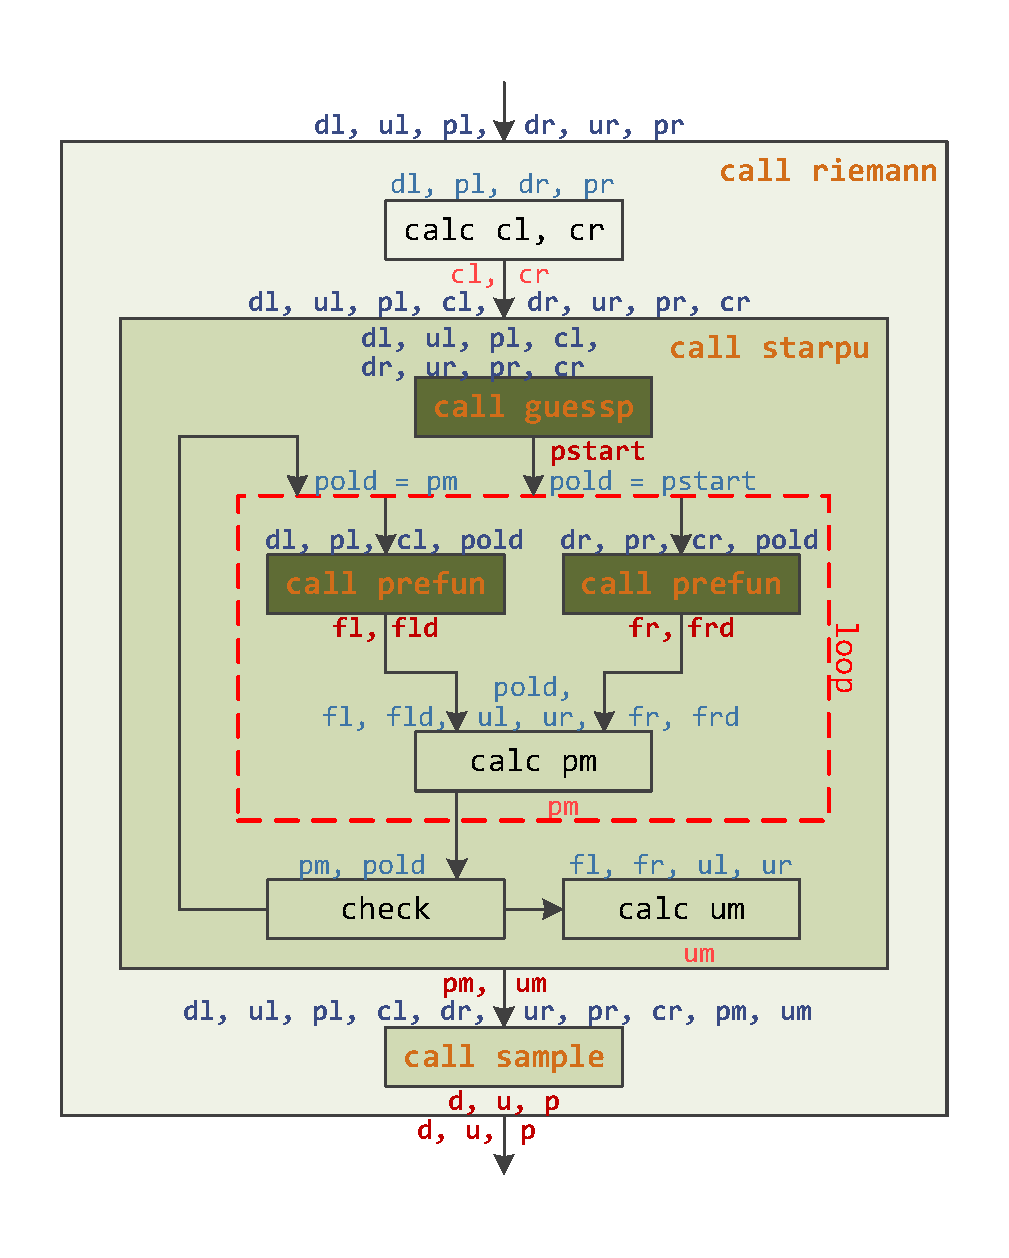
\includegraphics[width=8cm]{pics/pic_functions}
\caption{Схема потока данных в римановском решателе}
\label{pic:functions}
\end{figure}

На Рис.~\ref{pic:functions} показана схема работы римановского решателя с обозначенными потоками данных и вызовами всех входящих в реализацию функций. Функция \texttt{riemann} осуществляет вычисление скорости звука справа и слева, выполняет проверку на образование вакуума и последовательно вызывает функции \texttt{starpu} и \texttt{sample}.
Функция \texttt{starpu} вычисляет значения скорости и давления в среднем регионе между левой и правой волнами (star region), при этом функция содержит цикл с неизвестным количеством итераций для решения нелинейного уравнения итерационным методом Ньютона, внутри которого расположены вызовы других функций (\texttt{prefun}).
Функции \texttt{guessp} и \texttt{prefun} содержат только арифметические вычисления и простые условия и являются наиболее простыми с точки зрения векторизации.
Наконец последняя функция sample определяет окончательную конфигурацию разрыва путем вычисления множества условий.
Данная функция содержит очень разветвленное управление, вложенность условий в ней достигает четырех, что затрудняет применение векторизации.

В процессе счета с помощью численных методов, базирующихся на римановском решателе, выполняется множество вызовов функции \texttt{riemann} с различными наборами входных данных (на каждой итерации счета выполняется один вызов для каждой грани каждой ячейки расчетной сетки).
Так как функция riemann является чистой, то вызовы для разных наборов входных данных (\texttt{dl}, \texttt{ul}, \texttt{pl}, \texttt{dr}, \texttt{ur}, \texttt{pr}) являются независимыми и возникает желание объединения вызовов с целью эффективного задействования векторных (поэлементных) инструкций.
В качестве такого объединенного вызова будем рассматривать функцию, в которую вместо атомарных данных типа \texttt{float} будут подаваться соответствующие векторы, содержащие по 16 элементов.

\begin{equation}\label{eq:riemann_16}
\overline{U_l} = \left( \begin{array}{ccc} \overline{d_l} \\ \overline{u_l} \\ \overline{p_l} \end{array} \right),
\overline{U_r} = \left( \begin{array}{ccc} \overline{d_r} \\ \overline{u_r} \\ \overline{p_r} \end{array} \right),
\overline{U} = \left( \begin{array}{ccc} \overline{d} \\ \overline{u} \\ \overline{p} \end{array} \right) = riem(\overline{U_l}, \overline{U_r})
\end{equation}

В формуле (\ref{eq:riemann_16}) все переменные $\overline{d_l}$, $\overline{u_l}$, $\overline{p_l}$, $\overline{d_r}$, $\overline{u_r}$, $\overline{p_r}$, $\overline{d}$, $\overline{u}$, $\overline{p}$ являются векторами длины 16.
Например, вектор $\overline{d}$ содержит 16 значений плотности газа, полученных при решении 16 задач Римана, объединенных в один вызов.
Аналогично с другими переменными.

При этом с векторными данными можно производить те же действия, что и с базовыми типами -- выполнять вычисления, передавать в функции, возвращать в качестве результата.
В процессе оптимизации для наглядности будем избегать подстановки тела функции в точку вызова.
Таким образом, в результате векторизации нашей целью является получение векторных аналогов всех используемых в римановском решателе описанных выше функций.

\section{Векторизация простого контекста}

Наиболее простым контекстом для векторизации вычислений при объединении вызовов является функция \texttt{prefun} (функция \texttt{guessp} обладает похожими свойствами и не рассматривается).
Невекторизованный вариант функции представлен на Рис.~\ref{pic:prefun_code}.

\begin{figure}
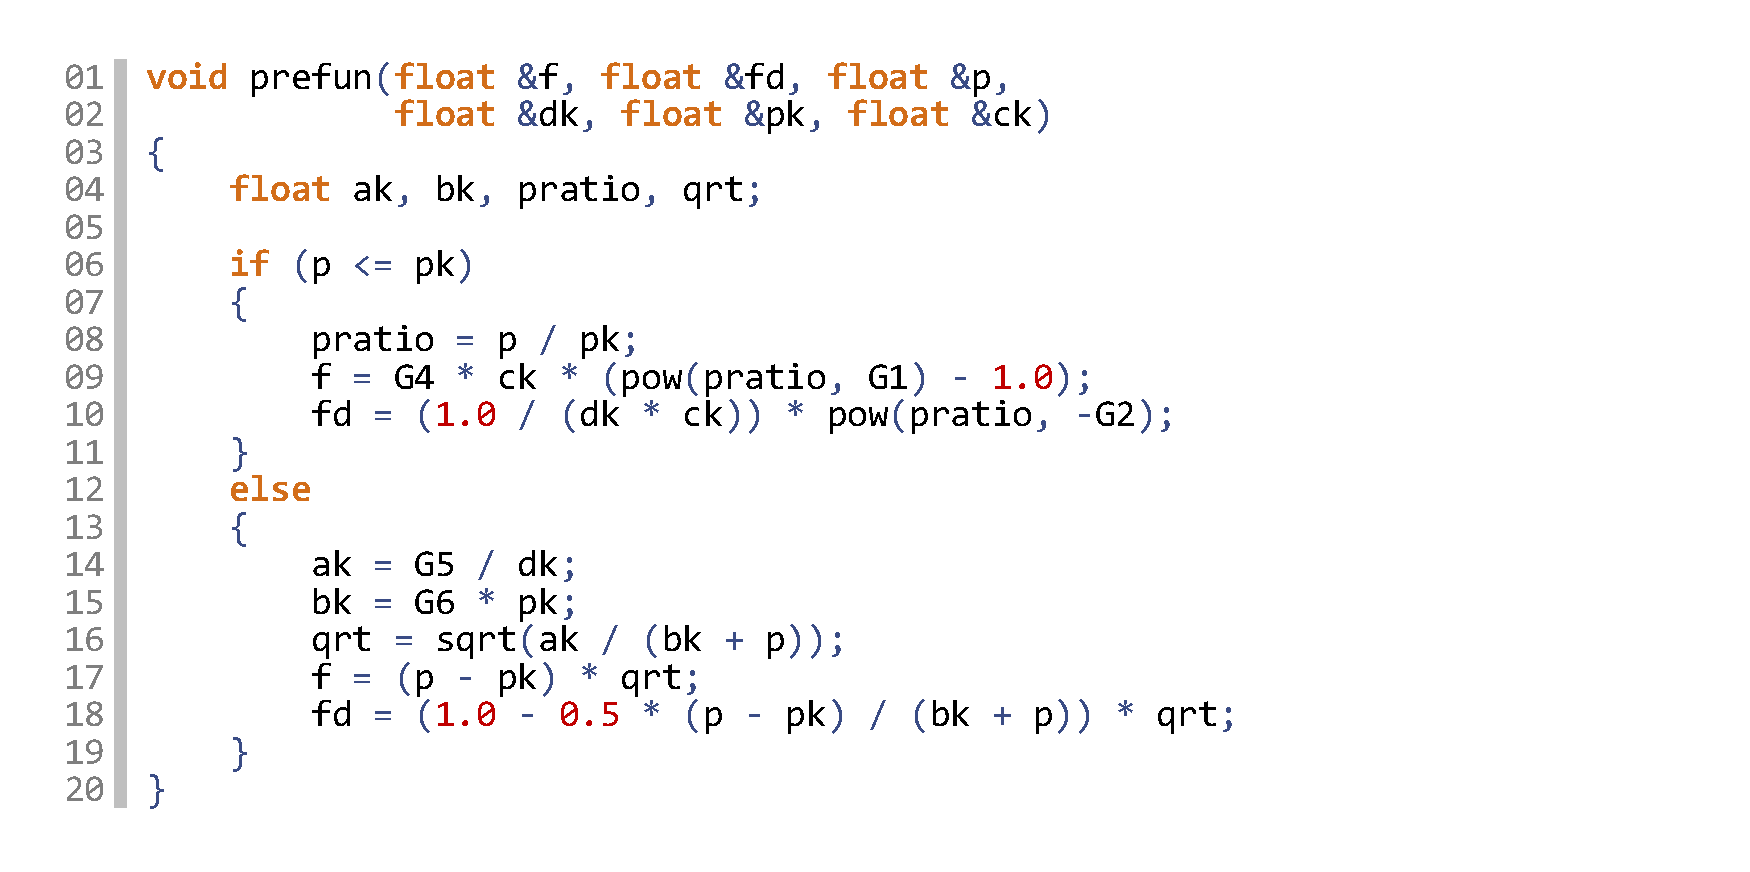
\includegraphics[width=10cm]{pics/pic_prefun_code}
\caption{Оригинальная версия функции \texttt{prefun}}
\label{pic:prefun_code}
\end{figure}

Данный код содержит только простые арифметические операции, извлечение квадратного корня, возведение в степень и сравнение.
Для всех этих действий в наборе команд AVX-512 предусмотрены векторные аналоги.
Код функции векторизуется путем замены арифметических операций на векторные аналоги.
Вычисление значений, находящихся под условием (\texttt{if-else}) векторизуется путем использования векторных предикатов, полученных с помощью векторного сравнения (см. Рис.~\ref{pic:prefun_16_code}).
В проведенной векторизации функции \texttt{prefun} стоит отметить три момента.

\begin{figure}
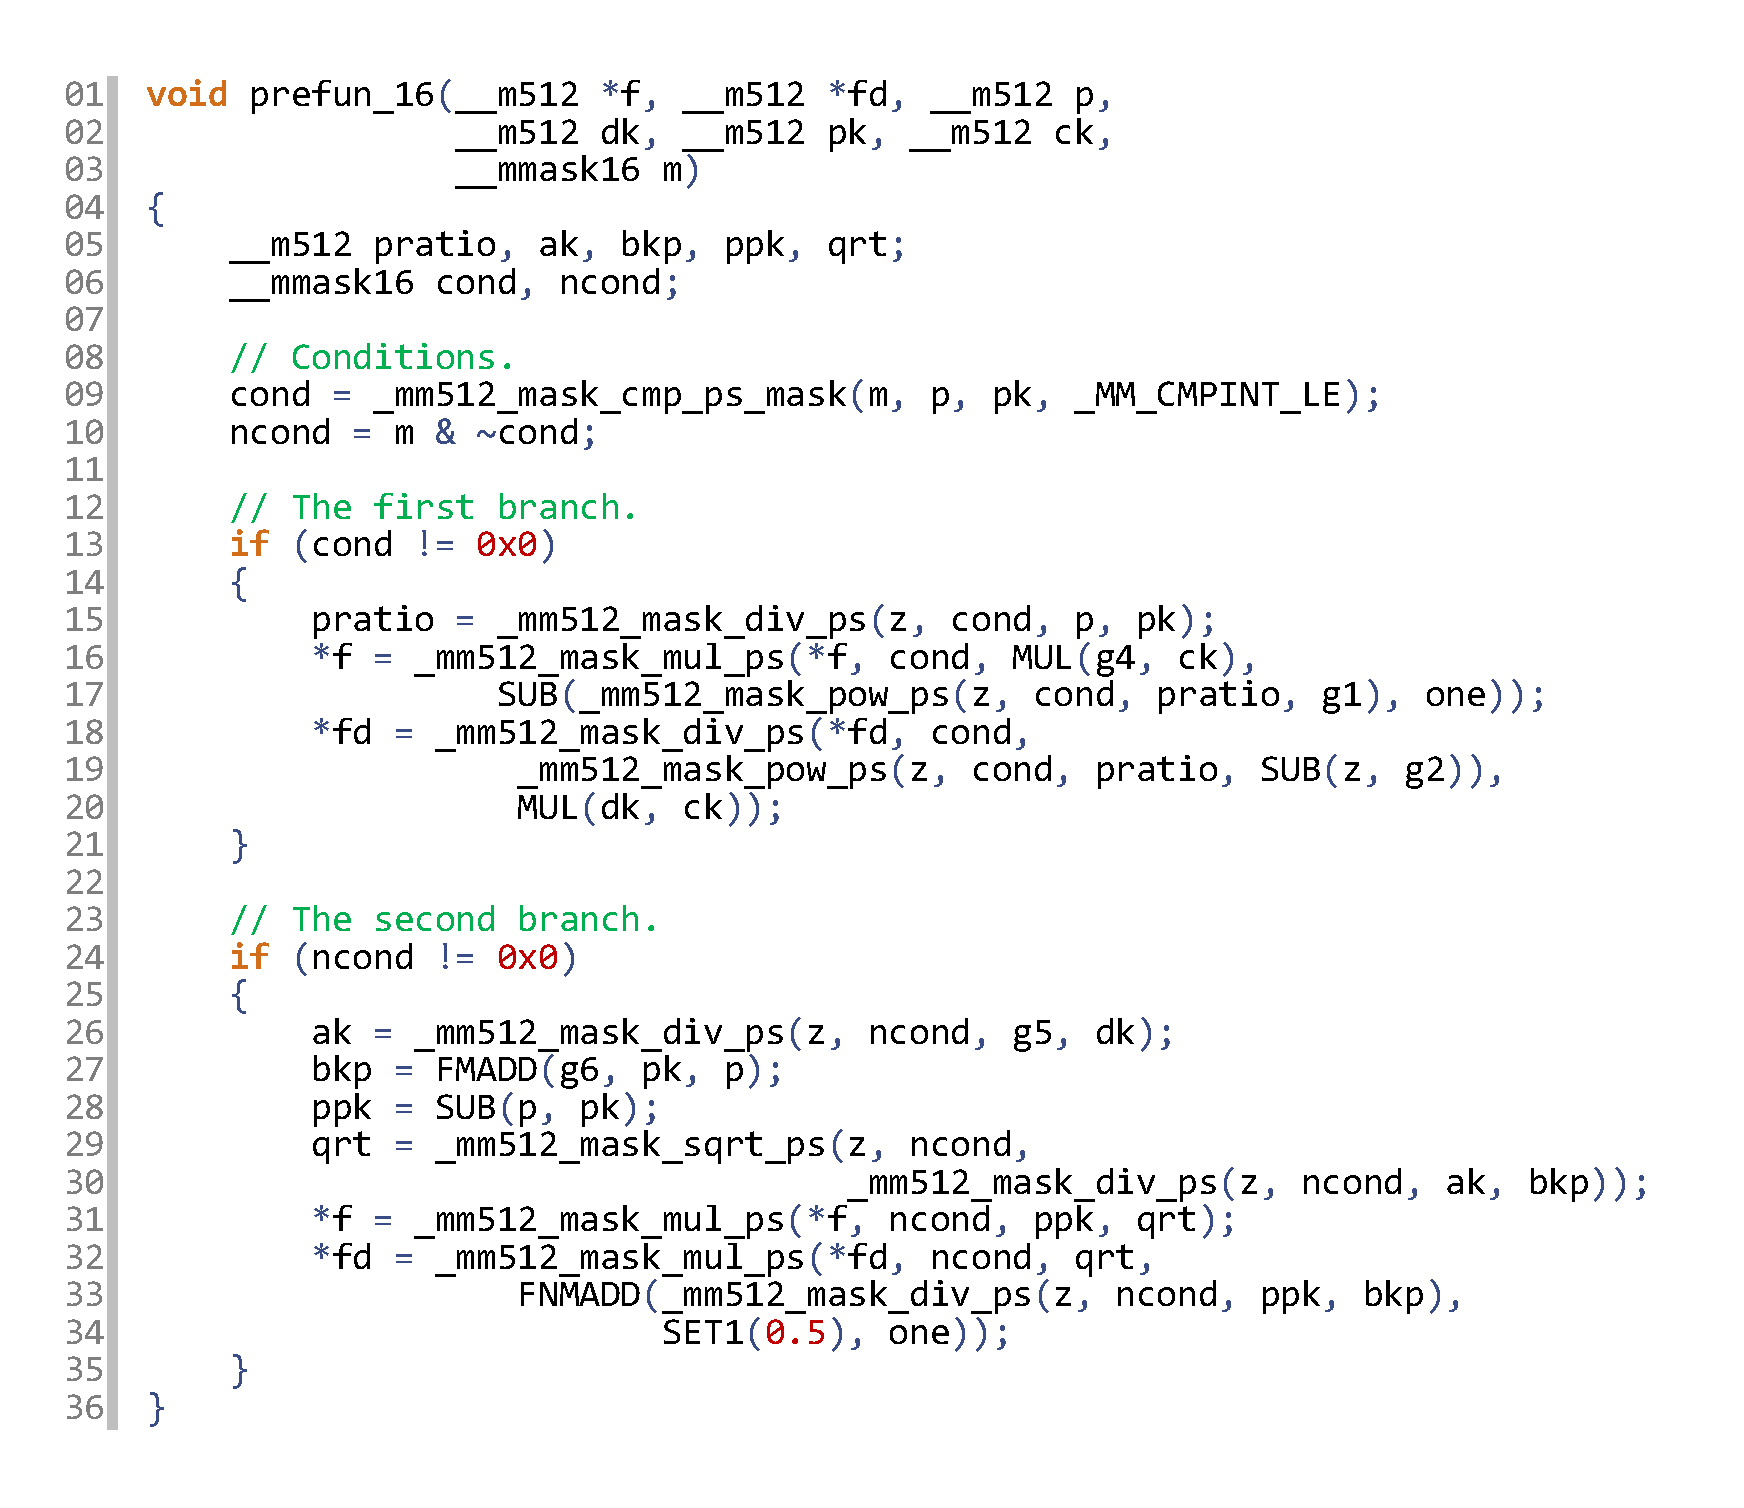
\includegraphics[width=10cm]{pics/pic_prefun_16_code}
\caption{Векторизованная версия функции \texttt{prefun}}
\label{pic:prefun_16_code}
\end{figure}

Так как векторная операция деления является медленной, то использовались следующие тождества для сокращения количества делений:

\begin{equation}\label{eq:deldel}
\frac{a}{\frac{b}{c}} = \frac{ac}{b}, \frac{\frac{a}{b}}{c} = \frac{a}{bc}
\end{equation} 

Так как функция \texttt{prefun} вызывается внутри цикла в функции \texttt{starpu}, то в ее реализацию необходимо добавить дополнительный аргумент-маску, по которой выбираются элементы, обрабатываемые в данном вызове (Рис.~\ref{pic:prefun_16_code}, строка 03).
Более подробно это будет описано ниже, когда будет обсуждаться векторизация функции \texttt{starpu}.

Еще одним важным моментом векторизации является оптимизация работы с условиями.
В процессе выполнения векторизации у нас сформировались две группы векторных инструкций, выполняемых под предикатами \texttt{cond} (Рис.~\ref{pic:prefun_16_code}, строки 15-20) и \texttt{ncond} (Рис.~\ref{pic:prefun_16_code}, строки 26-34).
Так как для физических задач характерно непрерывное изменение физических величин, то можно утверждать, что наборы данных, обрабатываемых в векторизованном вызове, близки.
Другими словами, все векторы, фигурирующие в вычислениях, содержат близкие значения.
Это же утверждение относится и к векторам предикатов.
Действительно, сбор статистики исполнения показал, что для физических задач наиболее частыми значениями векторов предикатов (в данном случае \texttt{cond} и \texttt{ncond}) являются значения \texttt{0x0} и \texttt{0xFFFF}.
Таким образом, проверки предикатных векторных регистров на пустоту (Рис.~\ref{pic:prefun_16_code}, строки 13 и 24) сразу отсекает целые блоки лишних операций, выполняемых с нулевой маской.

\section{Векторизация сильно разветвленных условий}

\begin{figure}
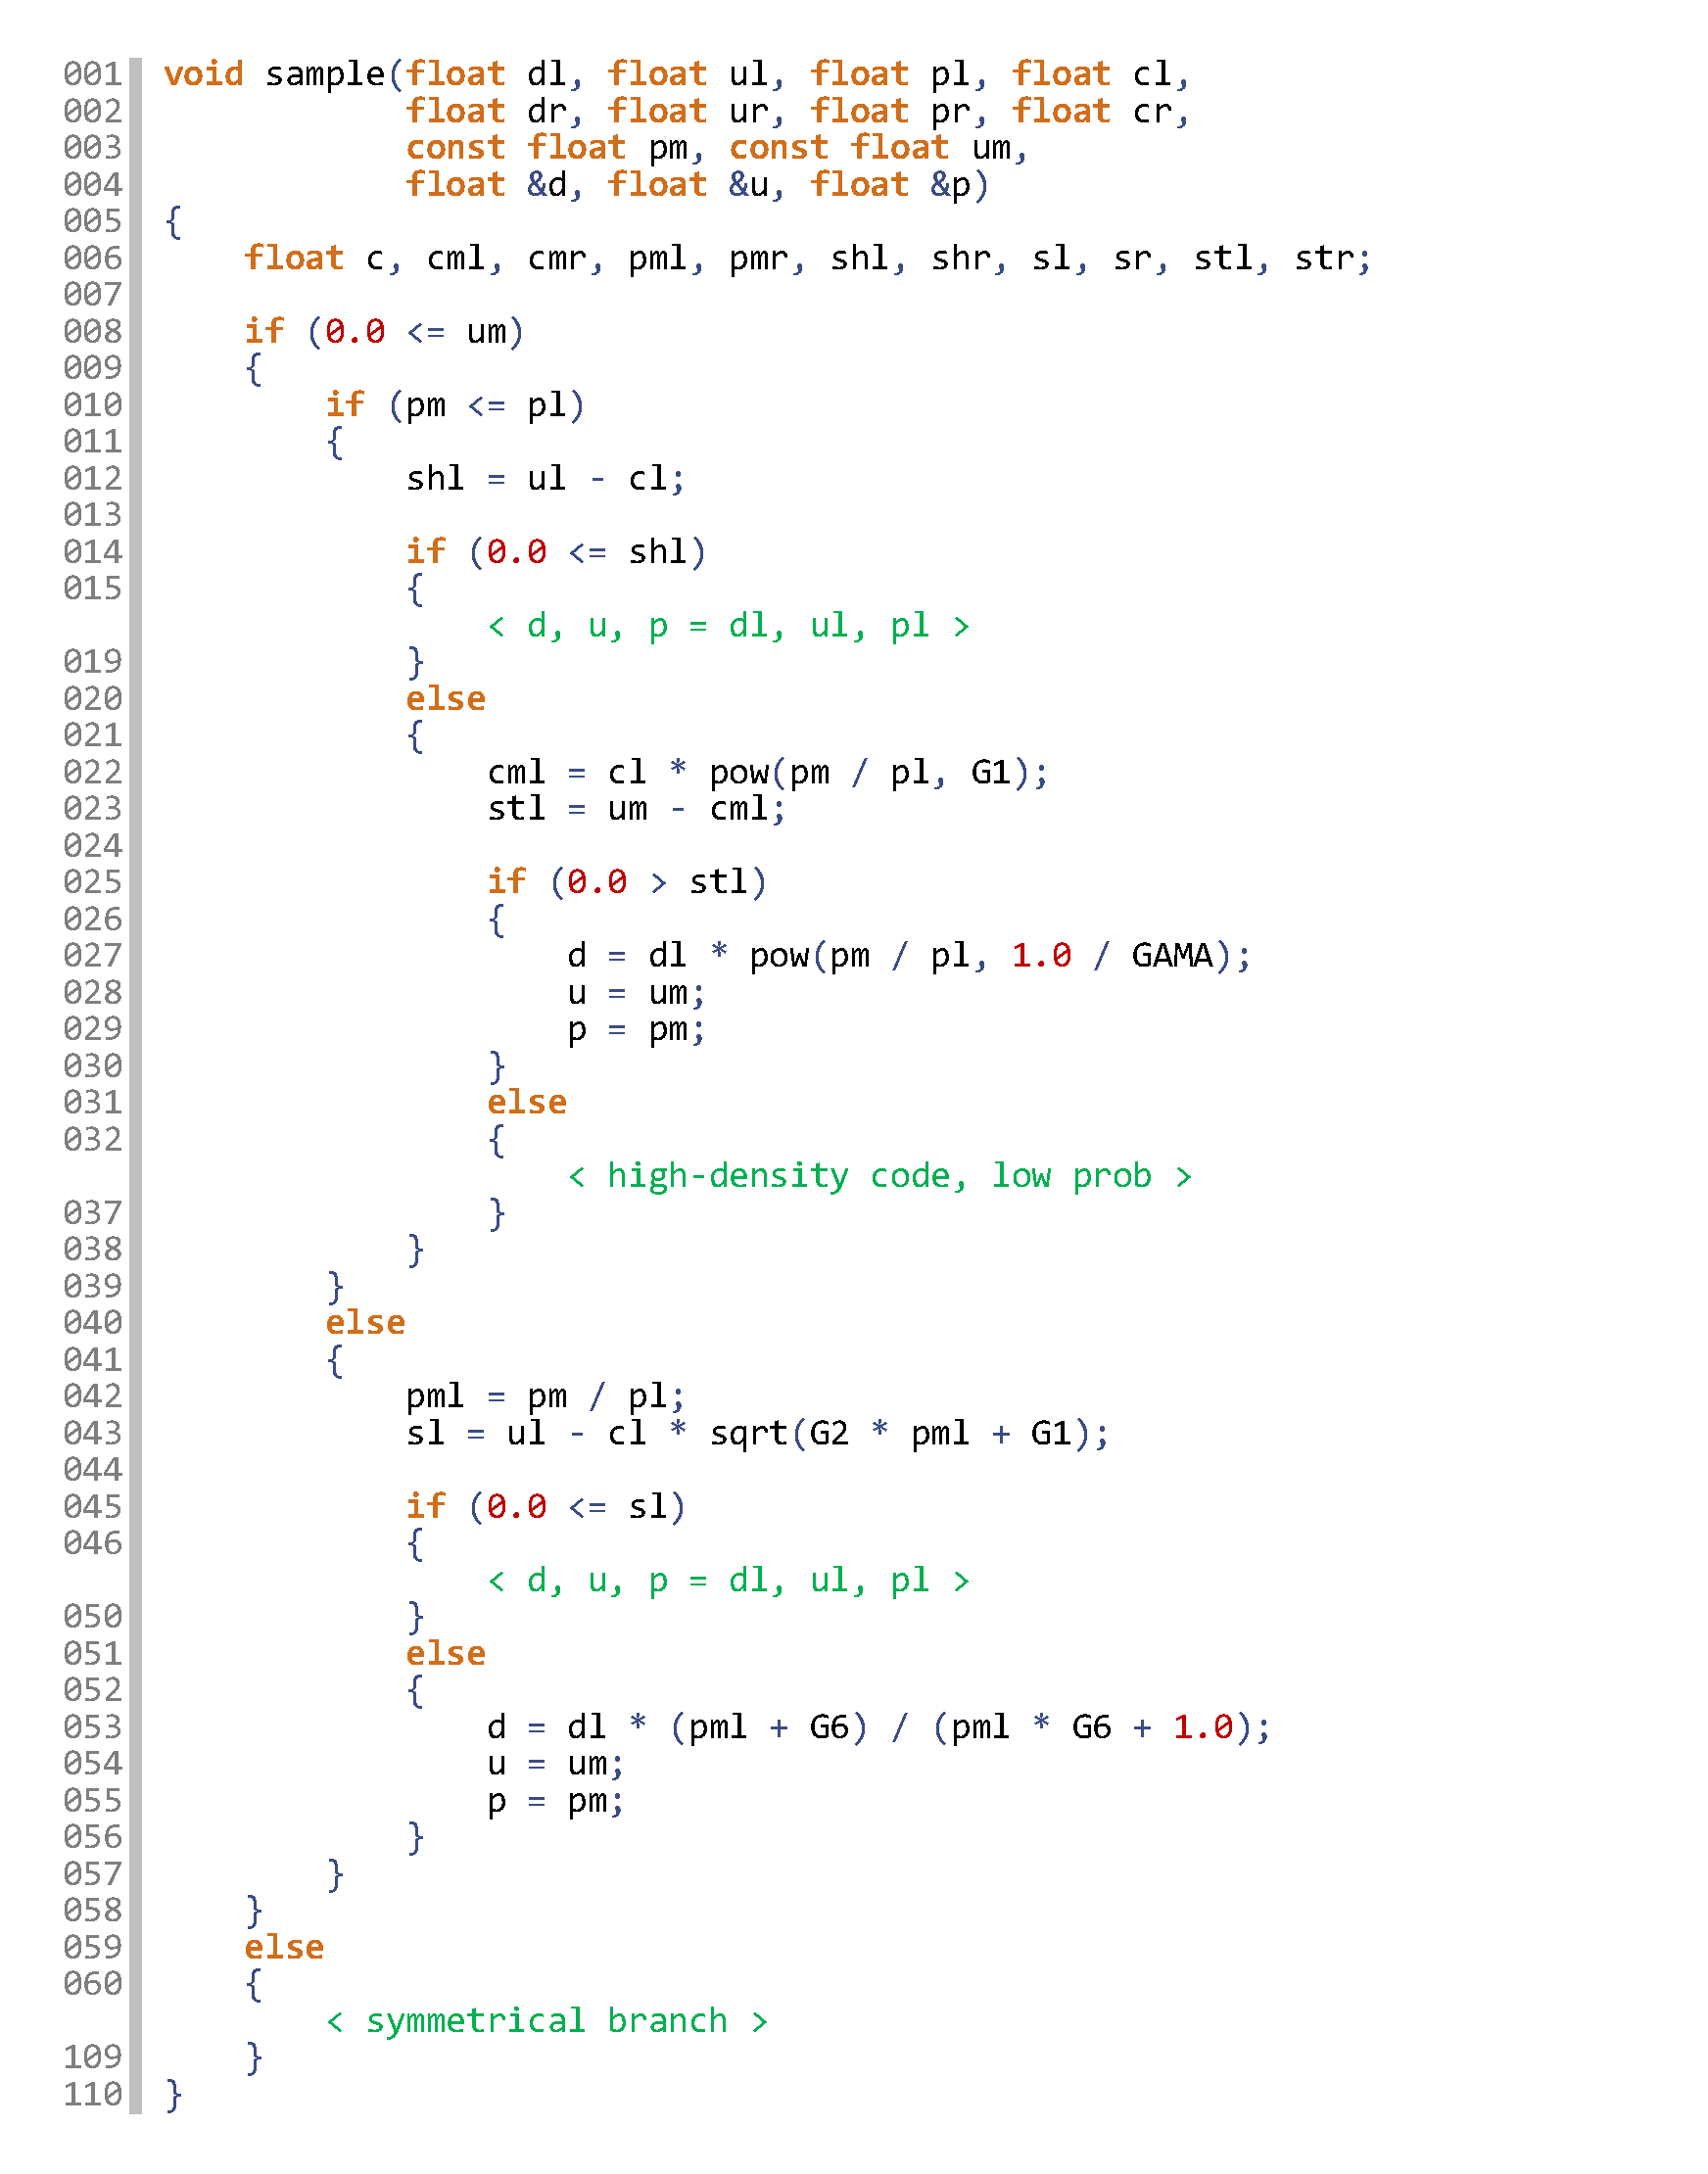
\includegraphics[width=10cm]{pics/pic_sample_code_4}
\caption{Оригинальная версия функции \texttt{sample}}
\label{pic:sample_code_4}
\end{figure}

Функция \texttt{sample} содержит сильно разветвленное управление с уровнем вложенности условий, равным 4 (см. Рис.~\ref{pic:sample_code_4}).
Дерево условий, построенное для данной функции содержит 10 листовых узлов, в каждом из которых определяется значение газодинамических величин \texttt{d}, \texttt{u}, \texttt{p}.
Прямое вычисление векторных предикатов всех листовых узлов и выполнение их кода под этими предикатами приводит к замедлению результирующего кода, поэтому при векторизации данной функции выполнялись следующие действия.

Во-первых, было замечено, что 4 линейных участка содержат определение газодинамических параметров \texttt{d}, \texttt{u} и \texttt{p}, которое можно было изменить на инициализацию с помощью выноса операций присваивания вверх по коду функции.
Таким образом, 4 линейных участка были удалены.
При этом данная инициализация параметров \texttt{d}, \texttt{u}, \texttt{p} не содержит арифметических операций (параметры инициализируются аргументами функции \texttt{dl}, \texttt{ul}, \texttt{pl} или \texttt{dr}, \texttt{ur}, \texttt{pr}), а значит может быть выполнена с помощью векторных операций слияния \texttt{blend}.

Далее было отмечено, что функция \texttt{sample} обрабатывает одинаковым образом правый и левый профиль распада разрыва с незначительными изменениями.
С помощью простой замены переменных, заключающейся в изменении знака значения скорости, удалось выполнить слияние кода для двух поддеревьев, опирающихся на условие \texttt{pm} $\le$ \texttt{pl}, что позволило вдвое уменьшить объем расчетного кода и ожидаемо сократило время исполнения на 45\%. 

\begin{figure}
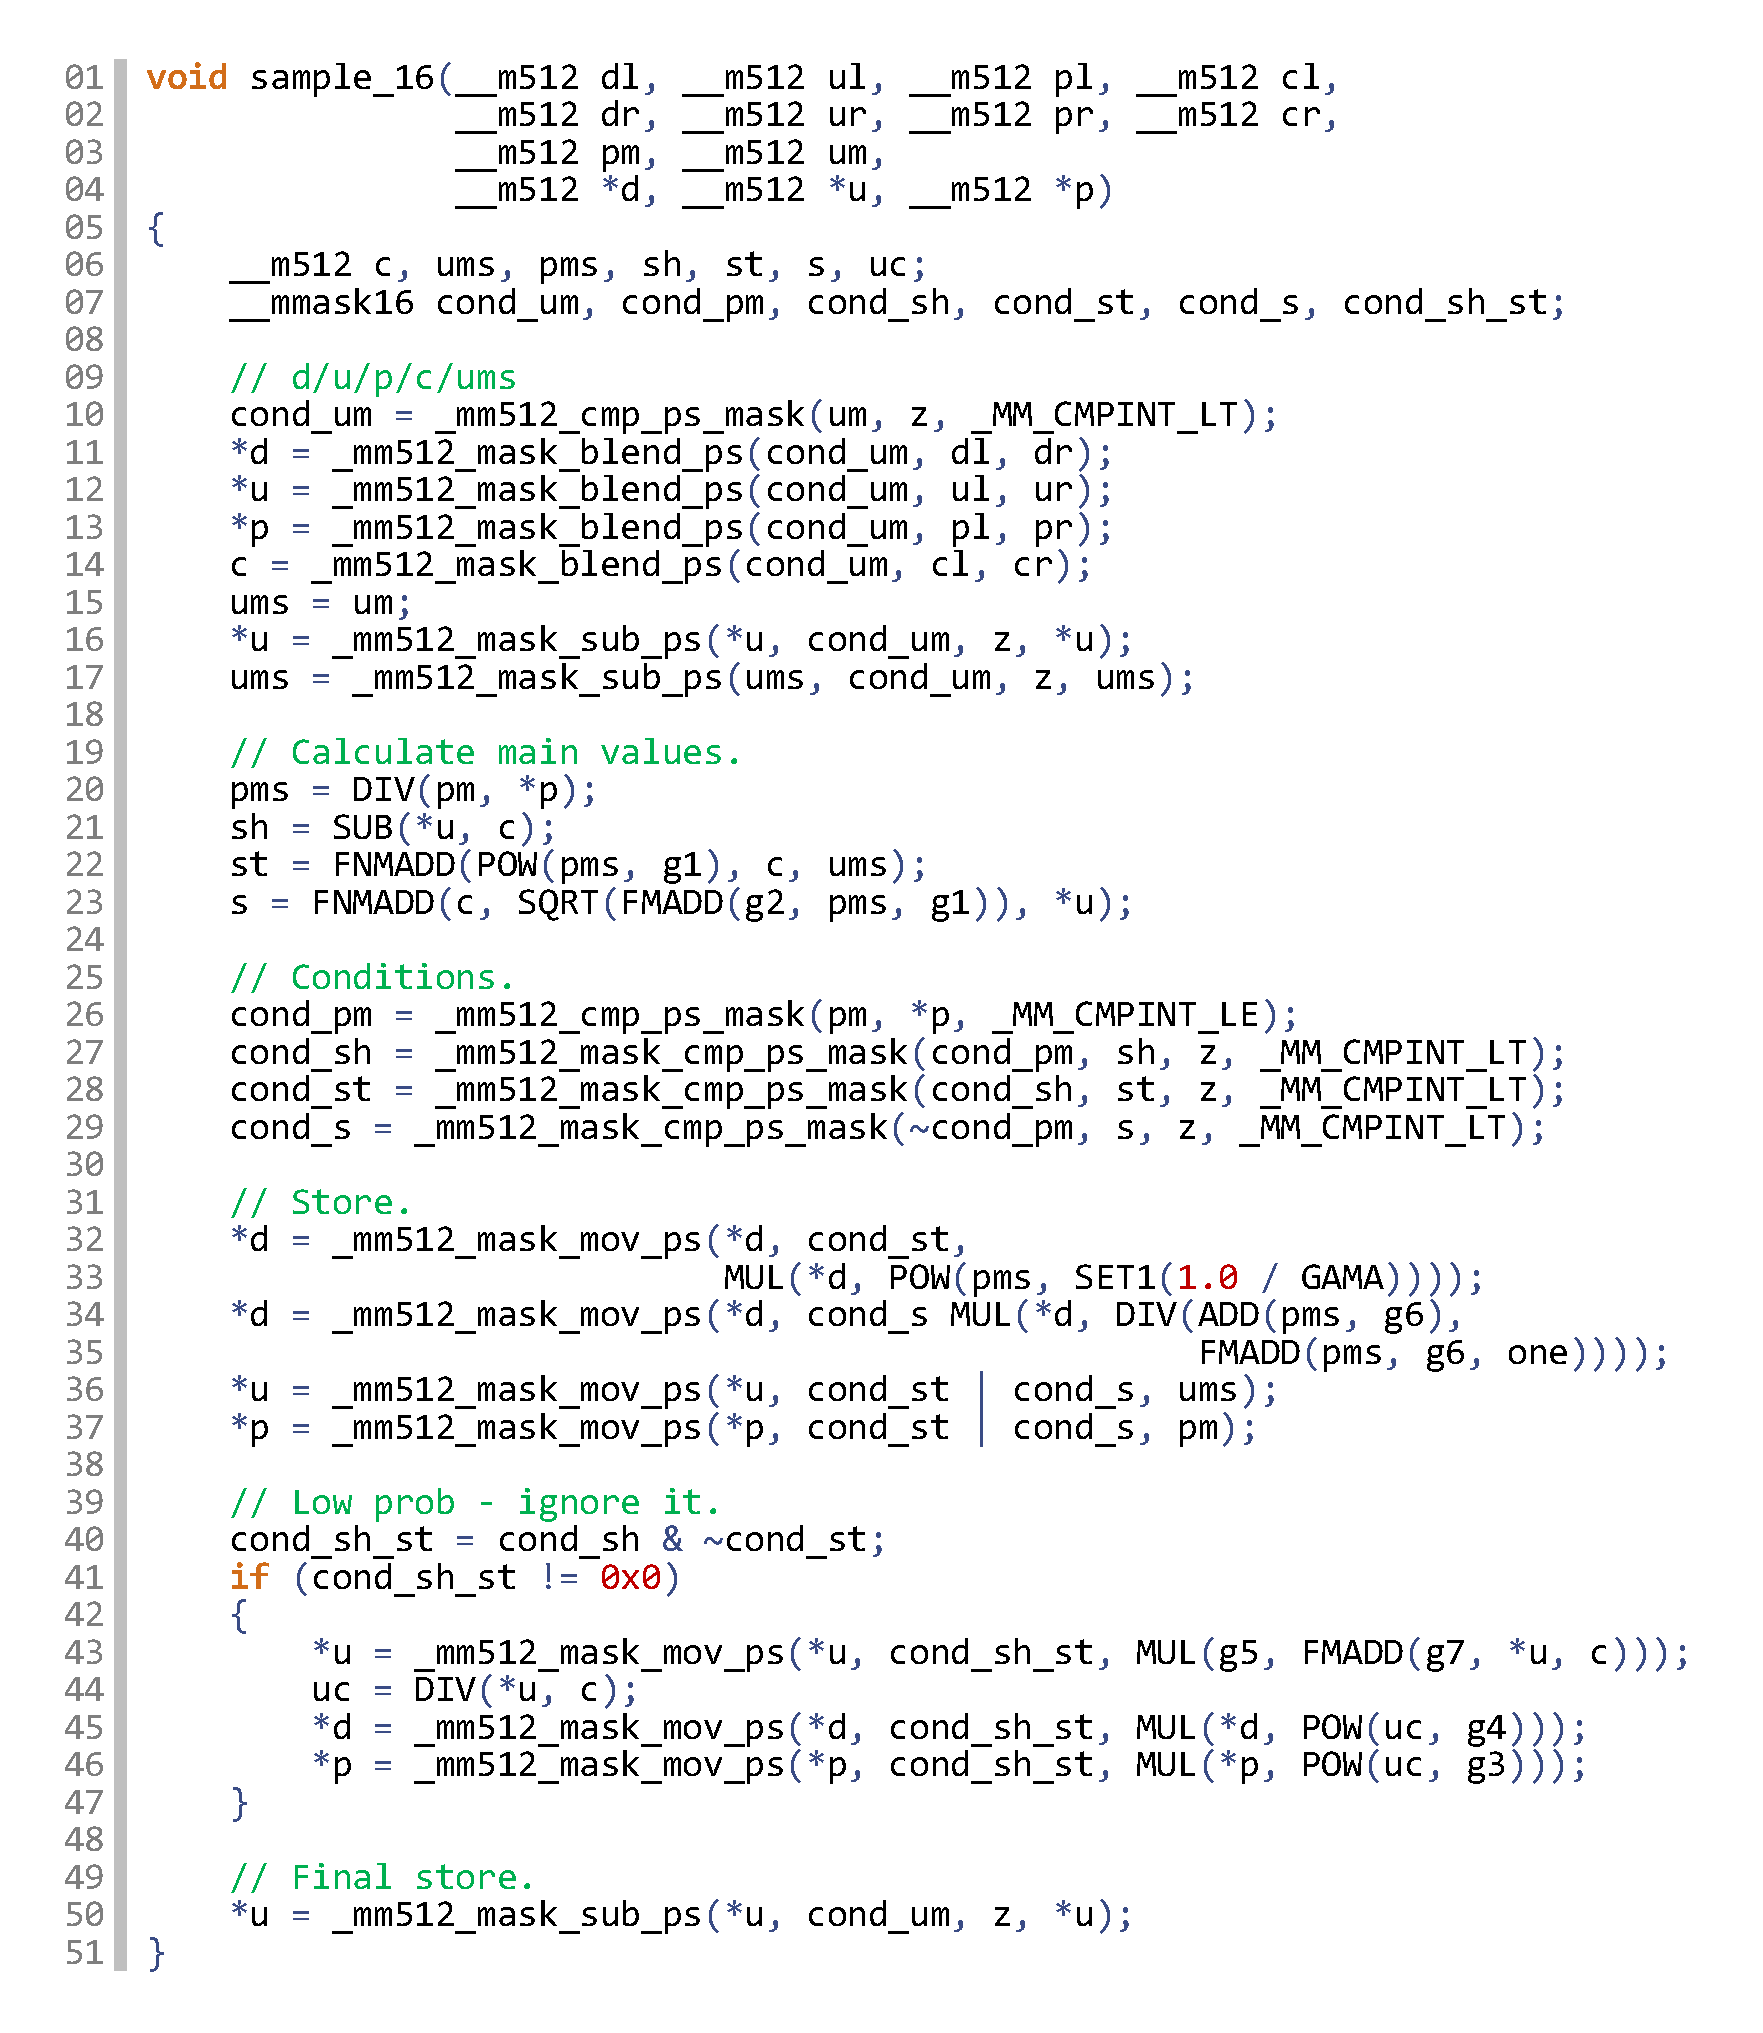
\includegraphics[width=10cm]{pics/pic_sample_16_code}
\caption{Векторизованная версия функции \texttt{sample}}
\label{pic:sample_16_code}
\end{figure}

После выполнения сокращения кода количество листовых узлов дерева условий сократилось до трех.
Однако даже в этом случае прямое слияние кода с использованием векторных предикатов оказалось неэффективным.
Виной тому послужил маловероятный участок кода, тяжелые операции, среди которых присутствуют вызовы функции возведения в степень (Рис.~\ref{pic:sample_code_4}, строки 033-036).
Векторный предикат данного участка кода более чем в 95 процентах случаев имеет значение \texttt{0x0}, поэтому перед выполнением данного участка кода целесообразно выполнить проверку данного предиката на пустоту (что соответствует выносу маловероятной ветви исполнения из тела функции).
Вынос маловероятной ветки исполнения из основного программного контекста способен существенно ускорить исполняемый код, так как наличие большого количества подобных редких вычислений может служить причиной к отказу от векторизации \cite{RybLowProb}.

Для остального кода можно производить слияние с учетом замечаний, описанных в предыдущем разделе.
В результате векторизованная функция \texttt{sample} была ускорена более чем в 10 раз.
Итоговый векторный код представлен на Рис.~\ref{pic:sample_16_code}.
В данном коде строки 11-14 соответствуют начальной инициализации, строки 16, 17 и 50 отвечают за замену переменных для слияния симметричных участков кода, а маловероятная ветка выделена в блоке, расположенном в строках 41-47.

\section{Векторизация гнезда циклов}

\begin{figure}
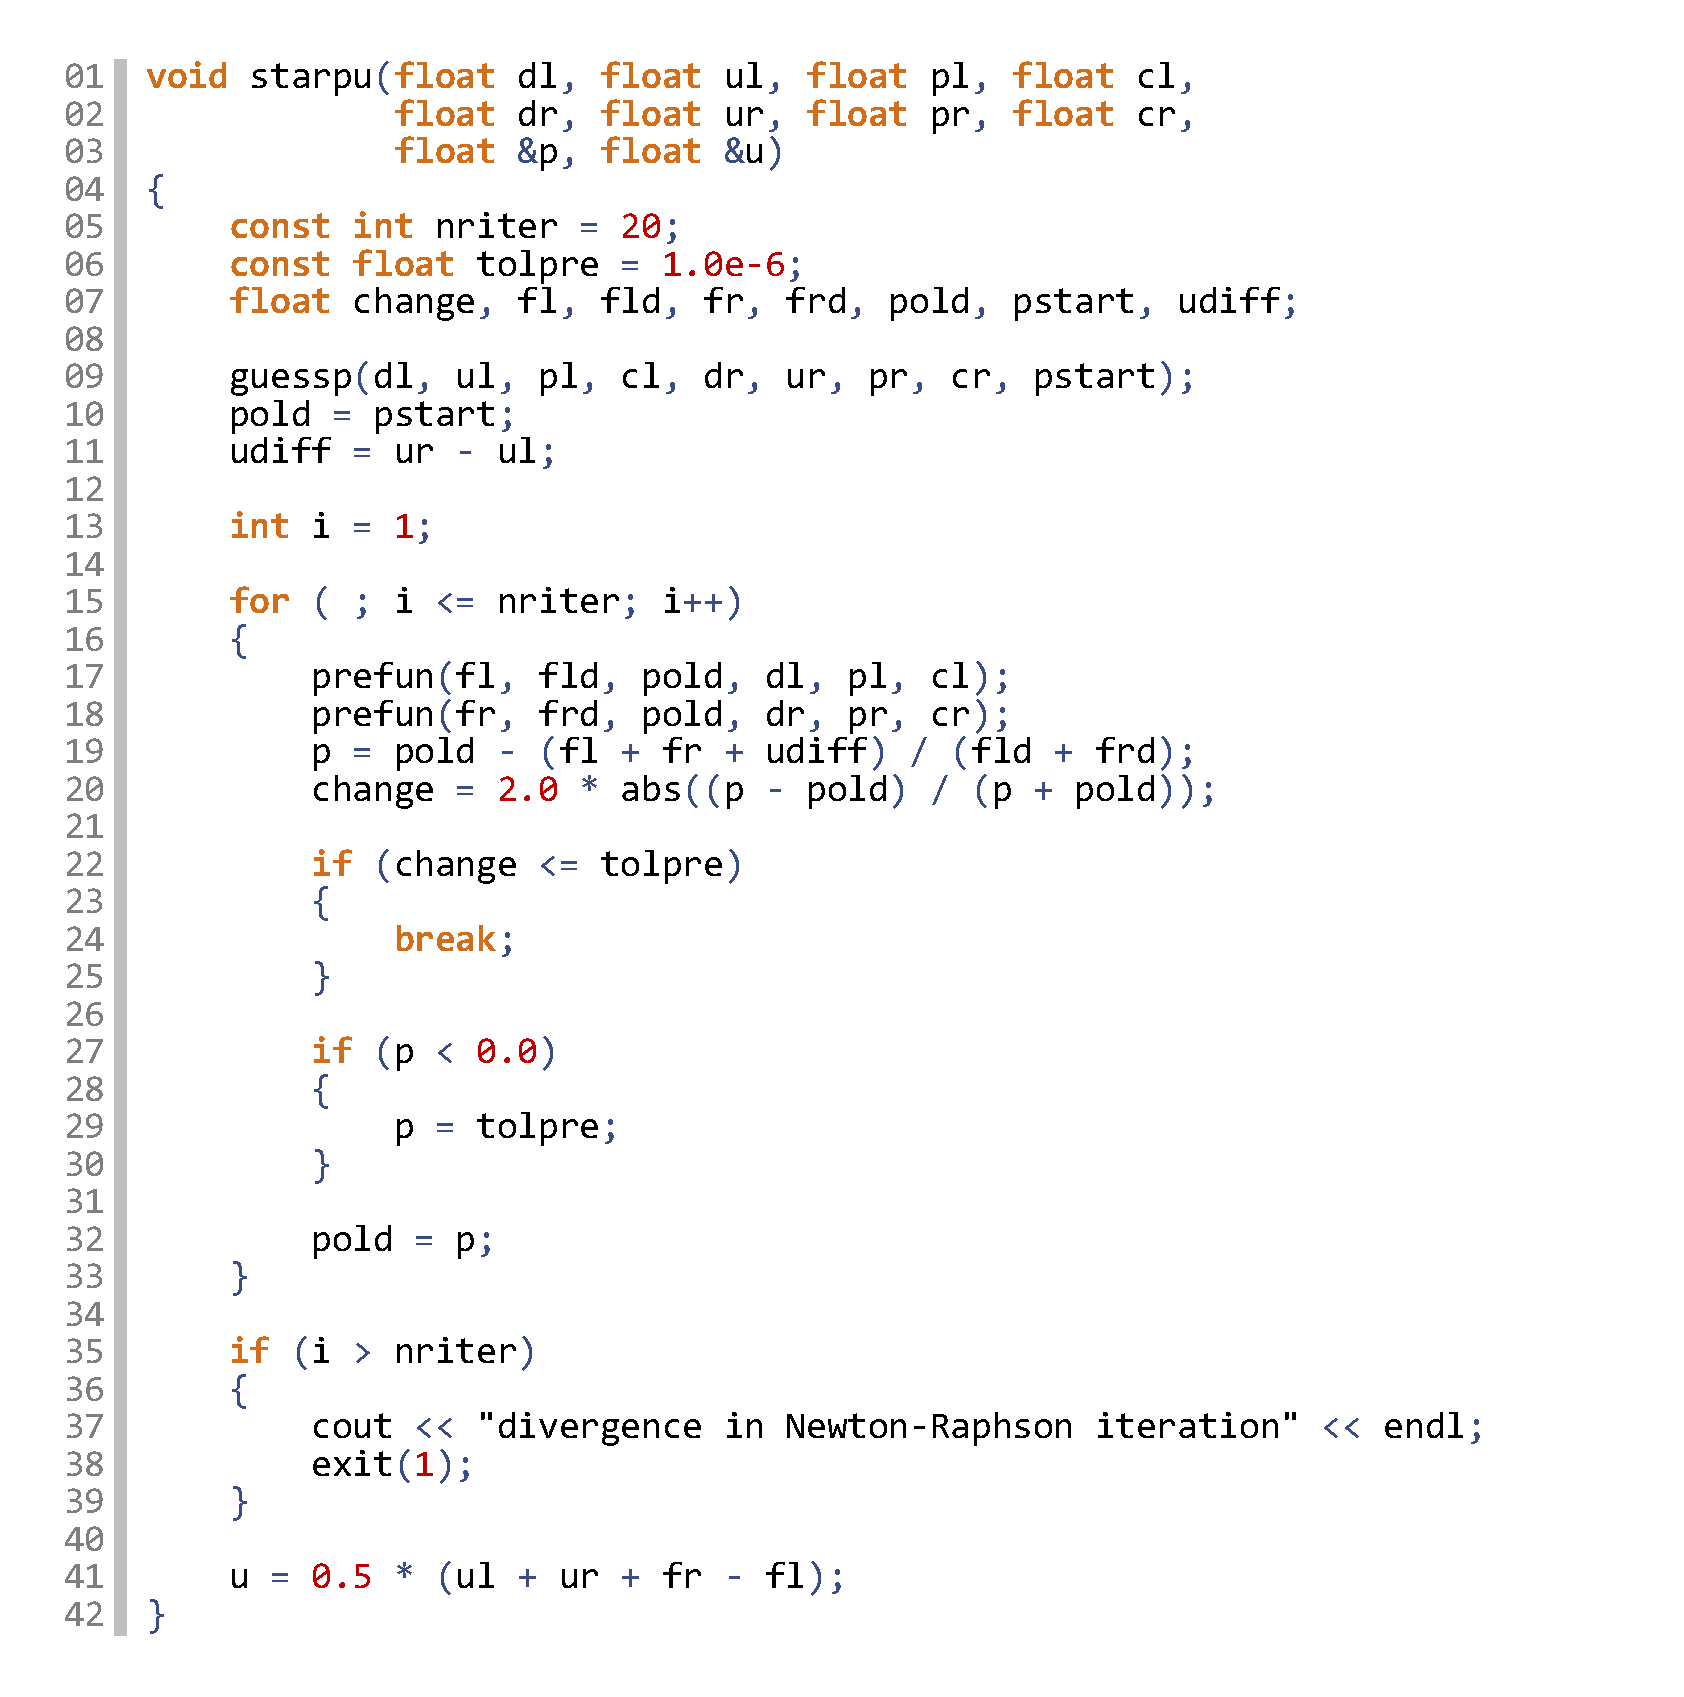
\includegraphics[width=10cm]{pics/pic_starpu_code}
\caption{Оригинальная версия функции \texttt{starpu}}
\label{pic:starpu_code}
\end{figure}

Наиболее сложным контекстом для векторизации кода является функция \texttt{starpu}, содержащая цикл с неизвестным количеством итераций (Рис.~\ref{pic:starpu_code}).
Цикл, расположенный в данной функции в строках 15-33 кроме неизвестного количества итераций содержит также условные переходы (\texttt{if, break}) и вызовы функций prefun, что также усложняет его векторизацию.
Перед выполнением векторизации данный цикл необходимо преобразовать в предикатную форму, в которой тело не должно содержать операций перехода.
Все инструкции цикла выполняются под своими предикатами, а выполнение цикла прерывается при условии обнуления всех предикатов.
Данный механизм описан в работе \cite{RybTelShabLoopsVect} применительно к векторизации сортировки Шелла, а также в \cite{Krzikalla} применительно к построению множества Мандельброта.
При этом стоит заметить, что вызовы функций prefun также должны обладать соответствующими предикатами.
После преобразования тела цикла в предикатную форму, он может быть векторизован, после чего предикаты инструкций заменятся на векторные регистры-маски (именно в этом месте появляется дополнительный параметр векторизованной функции \texttt{prefun} в виде маски).
Результат векторизации функции \texttt{starpu} представлен на Рис.~\ref{pic:starpu_16_code}.
В строке 18 видна изначальная инициализация полной маски выполнения векторизованных итераций цикла. По мере работы цикла маска истощается (строка 32), и при полном ее обнулении цикл завершает работу.

\begin{figure}
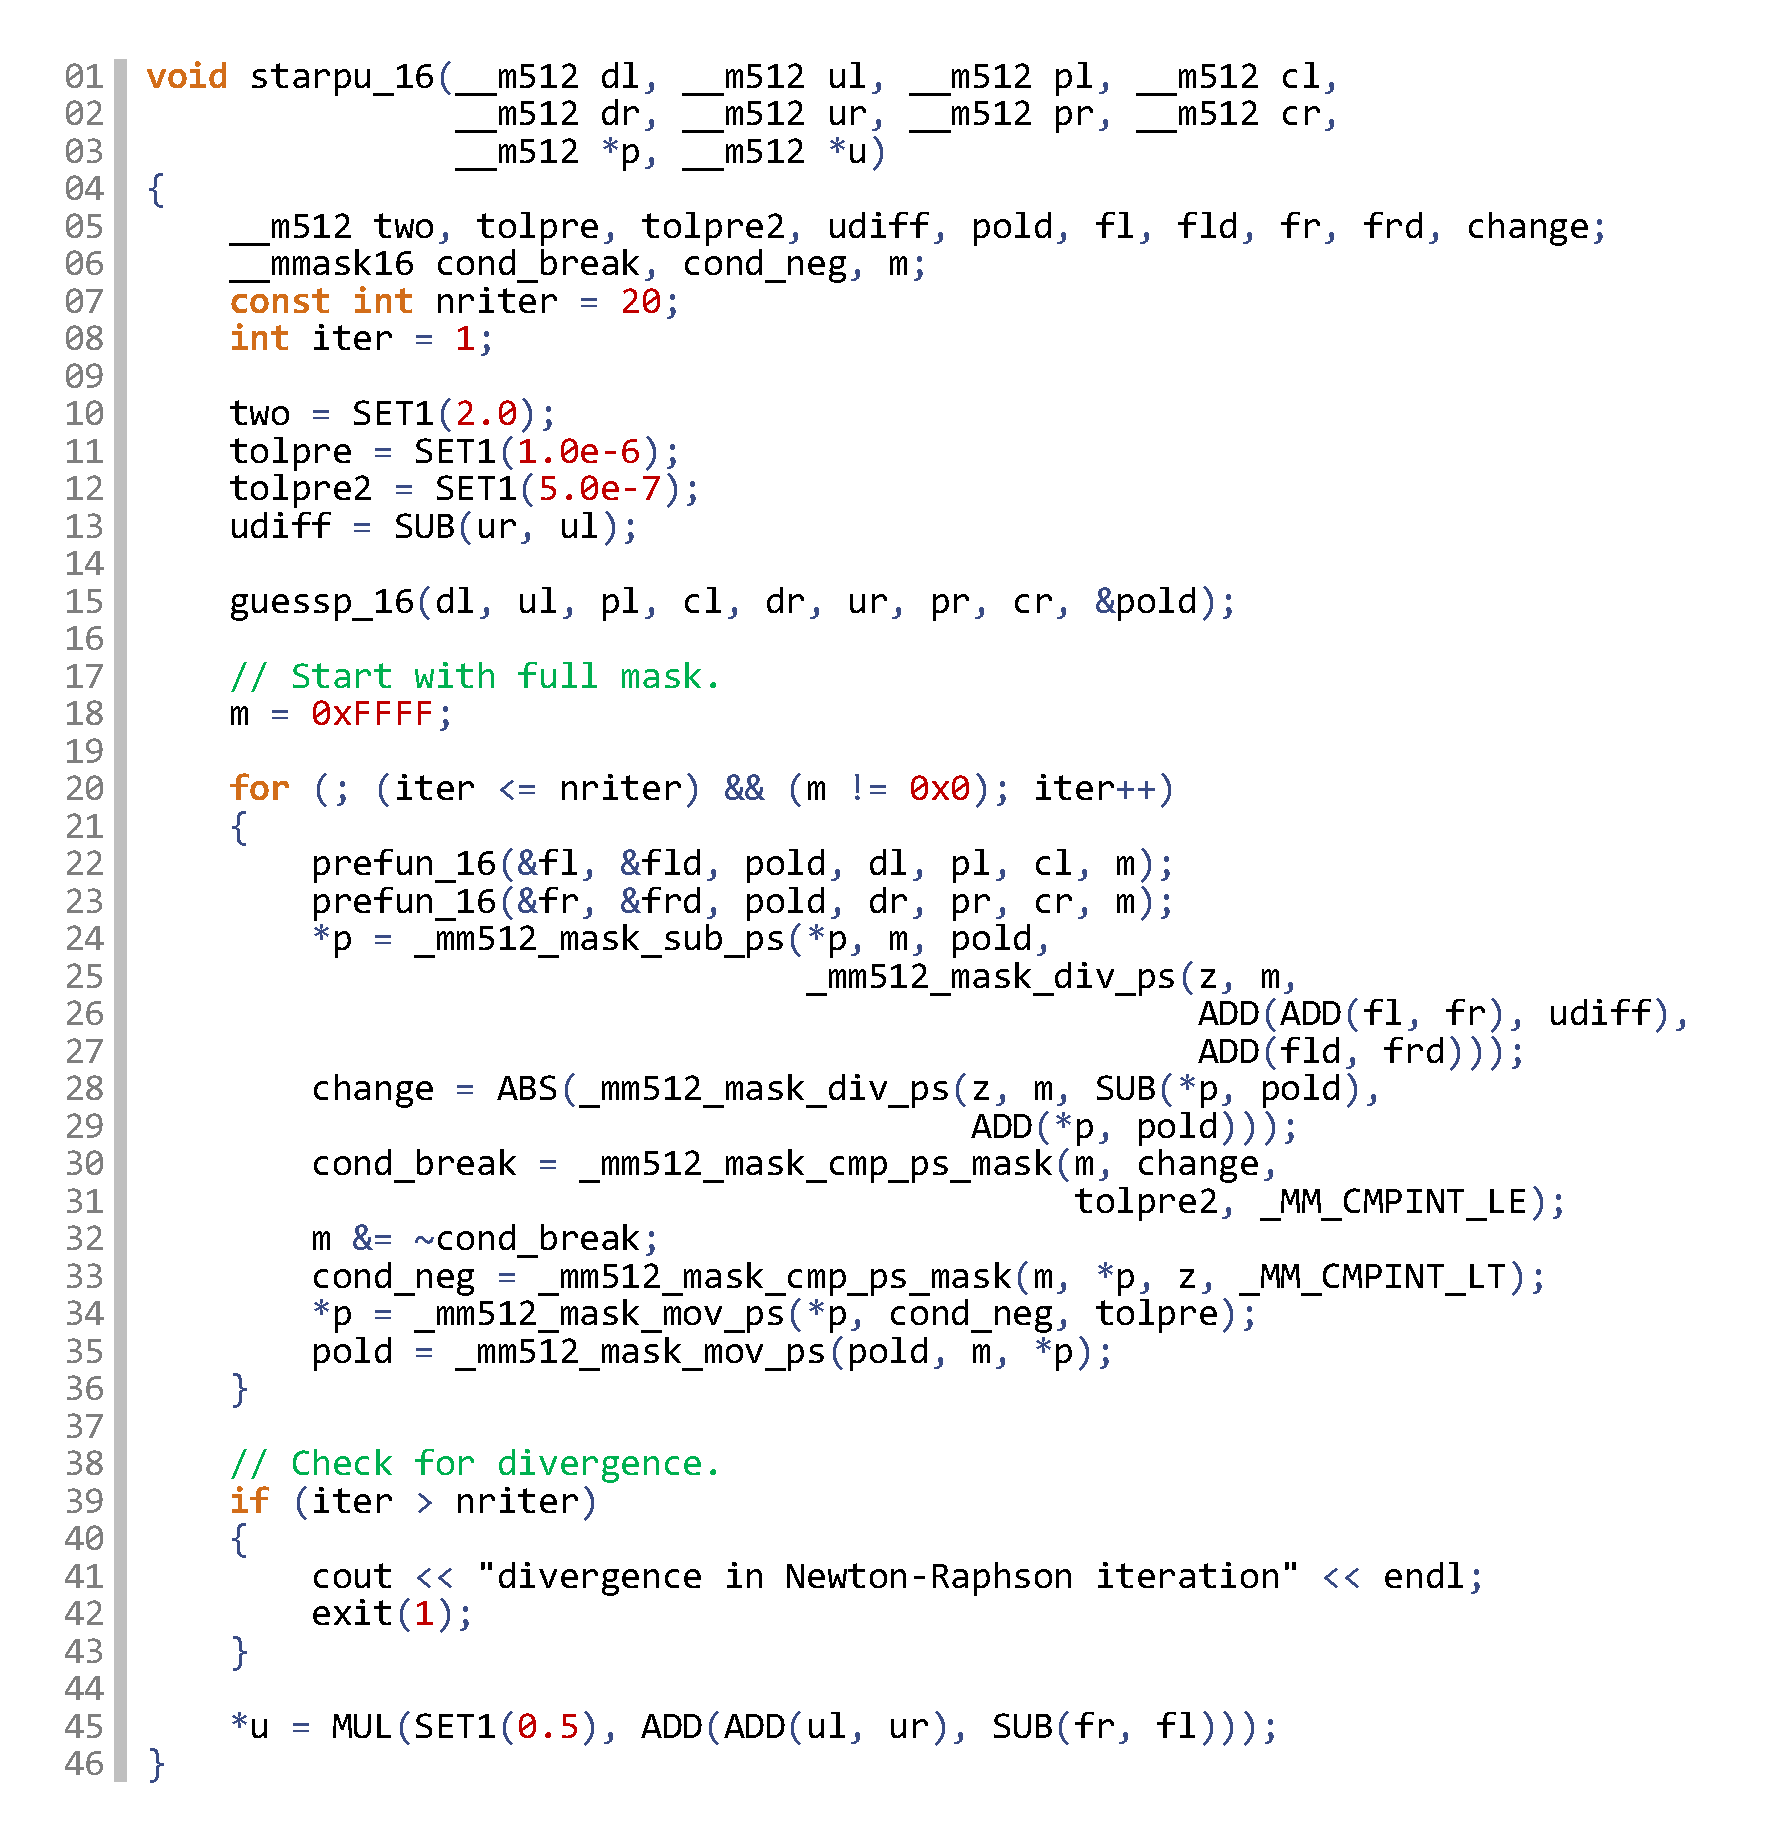
\includegraphics[width=10cm]{pics/pic_starpu_16_code}
\caption{Векторизованная версия функции \texttt{starpu}}
\label{pic:starpu_16_code}
\end{figure}

Стоит отметить, что векторизация цикла с неизвестным числом итераций может быть довольно опасной, так как количество итераций векторизованного цикла равно максимуму из количеств итераций циклов из 16 объединяемых вызовов оригинальной невекторизованной функции.
При большой разнице в количестве итераций оригинального кода возникает падение эффективности, связанное с низкой плотностью масок исполняемых инструкций, как это показано в работе \cite{RybTelShabLoopsVect}.

\section{Анализ результатов}

Перед началом оптимизации программного кода римановского решателя был выполнен сбор профиля исполнения, который показал, что время исполнения распределено между отдельными функциями согласно диаграмме, представленной на Рис.~\ref{pic:exe_prof}.

\begin{figure}
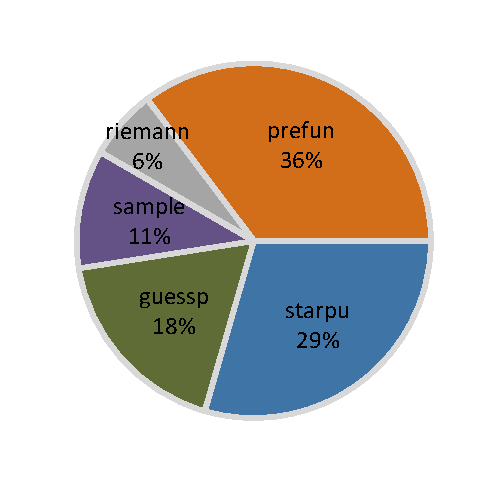
\includegraphics[width=8cm]{pics/pic_exe_prof}
\caption{Распределение времени выполнения римановского решателя между отдельными функциями}
\label{pic:exe_prof}
\end{figure}

Для сбора профиля исполнения исходная программа была скомпилирована с запретом оптимизации подстановки тела функции в точку вызова (inline).
Таким образом, на диаграмме отмечено чистое время выполнения функций без учета вложенных вызовов.
Из диаграммы видно, что наибольшая доля времени исполнения приходится на функцию \texttt{prefun} (36\%), содержащую простой программный контекст с одним условием.
Также значительная часть времени исполнения приходится на функцию \texttt{starpu} (29\%), содержащую гнездо циклов с неизвестным числом итераций.
Оставшееся время делится между тремя другими функциями \texttt{guessp} (18\%), \texttt{sample} (11\%), \texttt{riemann} (6\%).

Описанные в статье подходы к векторизации функций римановского решателя были реализованы на языке программирования C с использованием функций-инстринсиков и опробованы на микропроцессорах Intel Xeon Phi 7290, входящих в состав вычислительного сегмента knl суперкомпьютера МВС-10П, находящегося в МСЦ РАН.

Тестирование производительности выполнялось на массивах входных данных, собранных при решении стандартных тестовых задач: задача Сода, задача Лакса, задача о слабой ударной волне, задача Эйнфельдта, задача Вудворда-Колелла, задача Шу-Ошера и других \cite{BulVolTest}.
В результате выполненных преобразований исходного кода было достигнуто ускорение римановского решателя в 7 раз по сравнению с неоптимизированной версий.

На диаграмме Рис.~\ref{pic:perf} показан эффект от применения различных оптимизаций к каждой из рассматриваемых функций, а также суммарное ускорение, полученное вследствие векторизации.

\begin{figure}
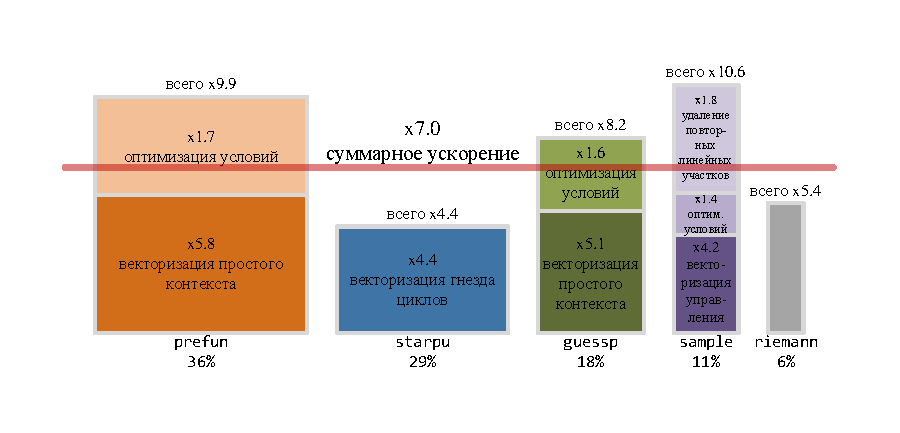
\includegraphics[width=12cm]{pics/pic_perf}
\caption{Диаграмма ускорения отдельных функций и суммарного ускорения римановского решателя}
\label{pic:perf}
\end{figure}

Можно отметить, что эффект от векторизации простого контекста варьируется в пределах от 5.1 до 5.8 раза (для функций \texttt{guessp} и \texttt{prefun}).
Также следует отметить существенный эффект от оптимизации условий (проверка на пустоту маски предикатов, под которой находится выполнение блока операций).
Это довольно простое преобразование, приводит к ускорению кода от 1.4 до 1.7 раз (для функций \texttt{sample} и \texttt{prefun}) в зависимости от того, насколько близкими являются условия с соседних итераций векторизуемого цикла.

Отдельно на диаграмме выделен эффект от применения оптимизации замены переменных, позволившей в 1.8 раз ускорить функцию \texttt{sample} путем слияния двух поддеревьев графа потока управления (то есть было выполнено удаление дублирующих линейных участков).

В результате применения всех описанных оптимизаций удалось достичь ускорения отдельных участков выполнения программы в 10 и более раз, а суммарное ускорение всего римановского решателя составило 7 раз (отмечено красной линией на Рис.~\ref{pic:perf}).

\section{Близкие работы}

Приведем краткое сравнение полученных в данной статье результатов с результатами других работ, направленных на повышение эффективности работы римановских решателей на параллельных архитектурах.
При этом отметим, что хотя в работе и не рассматривалось распараллеливание базирующихся на римановском решателе численных методов с помощью MPI, OpenMP, а также с помощью графических ускорителей, было бы неправильно не упомянуть работы, касающиеся данных аспектов распараллеливания.

В работе \cite{Shumlak} рассматривается алгоритм численного решения уравнений магнитной гидродинамики, базирующийся на приближенном римановском решателе Рое.
При этом вычисления проводятся на блочно-структурированной расчетной сетке, и для распараллеливания с помощью MPI выполняется декомпозиция блоков сетки (разрезание вдоль одного или нескольких направлений).
Приводятся результаты измерения показателя слабой масштабируемости при использовании до 16 процессоров.
Данный показатель оказывается близким к единице и даже в некоторых случаях превышает ее.
Такое явление, называемое сверхлинейной масштабируемостью, можно также встретить и в других работах, посвященных распараллеливанию численных методов газовой динамики, например в \cite{Benderskij}.

Работа \cite{Schive} посвящена распараллеливанию численных методов, базирующихся на различных приближенных римановских решателях, для выполнения на графических ускорителях NVIDIA Tesla C2050.
При этом кроме решателя Рое используются также решатели HLLE и HLLC \cite{Kong}.
Продемонстрированы методы, позволяющие достигнуть ускорения на графическом ускорителе по сравнению с процессором Intel Xeon E5530 в 101 раз при использовании равномерной сетки.
Также приведены показатели слабой и сильной масштабируемости распараллеленного приложения при использовании 32 GPU, они составили 98.8\% и 85.0\% соответственно. 

В работе \cite{Mandli} приведены результаты применения инструмента PetClaw (Python-оболочка, интегрирующая вычислительное ядро Clawpack, написанное на Fortran, и библиотеку PETSc в единое параллельное приложение) для распараллеливания гидродинамических расчетов с помощью MPI на большое количество ядер, вплоть до 16 тысяч.
При этом продемонстрирован близкий к единице показатель эффективности распараллеливания.

В работах \cite{Kulikov}, \cite{Kulikov2} описаны подходы к распараллеливанию вычислений при моделировании астрофизических течений на гибридных суперкомпьютерах, оснащенных ускорителями Intel Xeon Phi.
В частности было продемонстрировано 134-кратное ускорение расчетных кодов на одном ускорителе при использовании многопоточного распараллеливания, а также 75\% масштабируемость при использовании до 224 ускорителей.
В статье отмечено, что для дальнейшего ускорения приложения нужна векторизация вычислительного ядра и приводится прогноз по достижению 80\% пиковой производительности при условии применения векторизации.

Наиболее близкими к рассматриваемой работе являются \cite{BaderSWEVect}, \cite{FerreiraSWEVect}, в которых особое внимание уделяется векторизации римановского решателя для численного решения уравнений мелкой воды.
В работе \cite{BaderSWEVect} приведены результаты по ускорению 6-7 раз при векторизации римановского решателя на данный одинарной точности на ускорителях Intel Xeon Phi KNC.
В работе \cite{FerreiraSWEVect} метод векторизации был доработан и эффект составил уже 2.4-6.5 на операциях с двойной точностью на микропроцессорах Intel Xeon Phi KNL.
Однако в данных работах используется специально разработанный приближенный римановский решатель для уравнений мелкой воды \cite{George}.
Реализация этого решателя содержит более простой вычислительный контекст по сравнению с точным решателем, векторизация которого рассматривается в текущей работе.
Приближенный решатель из \cite{George} содержит только арифметические операции и поддается автоматической векторизации после специальной подготовки входных параметров (группировка нескольких вызовов решателя в один вызов с векторными параметрами).

Проведенное сравнение данной работы со схожими по тематике, позволяет заключить, что полученное с помощью набора инструкций AVX-512 значение ускорения точного римановского решателя равное 7, является хорошим результатом.

\section*{Заключение}

В работе были рассмотрены подходы к векторизации сложного программного контекста с помощью использования набора инструкций AVX-512.
Данный набор инструкций появился в микропроцессорах Intel начиная с ускорителей Intel Xeon Phi KNC, а затем вошел в микропроцессоры Intel Xeon Phi KNL, Intel Xeon Phi Skylake и далее.
Инструкции AVX-512 поддерживают предикатную обработку элементов данных, что позволяет векторизовать с помощью них сложный разветвленный программный код.

В качестве целевой задачи был использован точный римановский решатель, так как он обладает компактной реализацией но в то же время содержит особенности, препятствующие автоматической векторизации средствами компилятора (вызовы функций, сложное управление, вложенные циклы).
Для векторизации использовался подход, при котором несколько последовательных вызовов функции решателя заменялись на один вызов с векторными параметрами (и с соответствующими изменениями тела функции).
Это позволило выполнять одновременно на одном процессорном ядре несколько экземпляров задачи (количество экземпляров равняется ширине вектора, в данном случае 16).

Были проанализированы составляющие части римановского решателя, выделены их особенности и для каждой из них предложен способ эффективной векторизации.
В результате векторизации было достигнуто ускорение более 10 раз на отдельных участках решателя, а итоговое ускорение составило 7 раз на данных с одинарной точностью.

Разработанные методы векторизации сложного программного контекста могут быть использованы для оптимизации других вычислительных задач.
В частности в настоящее время коллективом авторов данной статьи разрабатывается библиотека, направленная на векторизацию произвольных плоских циклов, то есть таких циклов, в которых отсутствуют межитерационные зависимости.
При этом тело цикла может включать такие элементы как сложное управление, гнезда циклов, вызовы чистых функций, операторы goto и другие.
Реализация такого инструмента позволит существенно повысить производительность расчетных кодов, автоматическая векторизация которых компилятором невозможна.

Работа выполнена в МСЦ РАН при поддержке гранта РФФИ №~18-07-00638. 

\begin{thebibliography}{30}

\RBibitem{KulPogSemRiemann}
\by А. Г. Куликовский, Н. В. Погорелов, А. Ю. Семенов
\book Математические вопросы численного решения гиперболических систем уравнений
\yr 2001
\publ ФИЗМАТЛИТ
\publaddr М.
\totalpages 608

\RBibitem{BorRykRiemann} 
\by В. Е. Борисов, Ю. Г. Рыков
\preprint Точный римановский солвер в алгоритмах решения задач многокомпонентной газовой динамики
\preprintinfo Препринты ИПМ им. М. В. Келдыша, № 96
\yr 2018 
\totalpages 28
\URL http://library.keldysh.ru/preprint.asp?id=2018-96
\crossref{http://dx.doi.org/10.20948/prepr-2018-96}

\RBibitem{Godunov}
\by С. К. Годунов, А. В. Забродин, М. Я. Иванов, А. Н. Крайко, Г. П. Прокопов
\book Численное решение многомерных задач газовой динамики
\yr 1976
\publ Наука
\publaddr М.
\totalpages 400

\RBibitem{Shumlak}
\by U. Shumlak, B. Udrea
\paper An approximate Riemann solver for MHD computations on parallel architectures
\jour Proceedings of the 15th AIAA Computational Fluid Dynamics Conference
\yr 2001
\crossref{http://dx.doi.org/10.2514/6.2001-2591}

\RBibitem{Schive}
\by H.-Y. Schive, U.-H. Zhang, T. Chiueh
\paper Directionally unsplit hydrodynamic schemes with hybrid MPI/OpenMP/GPU parallelization in AMR
\jour International Journal of High Performance Computing Applications
\yr 2011
\pages 367-377
\crossref{http://dx.doi.org/10.1177/1094342011428146}

\RBibitem{Mandli}
\by K. T. Mandly, A. Alghamdi, A. Ahmadia, D. I. Ketcheson, W. Scullin
\paper Using Python to construct a scalable parallel nonlinear wave solver
\jour Proceedings of the 10th Python in Science Conference (SCIPY 2011)
\yr 2011
\pages 61-66

\RBibitem{Kulikov}
\by И. М. Куликов, И. Г. Черных, Э. И. Воробьев, А. В. Снытников, Д. В. Винс и др.
\paper Численное гидродинамическое моделирование астрофизических течений на гибридных СуперЭВМ, оснащенных ускорителями Intel Xeon Phi
\jour Суперкомпьютерное моделирование
\yr 2016
\vol 5
\issue 4
\pages 77-97
\crossref{http://dx.doi.org/10.14529/cmse160406}

\RBibitem{Kulikov2}
\by I. Kulikov, I. Chernykh, V. Vshivkov, V. Prigarin, V. Mironov, A. Tatukov
\paper The parallel hydrodynamic code for astrophysical flow with stellar equation of state
\jour Proceedings of Russian Supercomputing Days 2018
\pages 612-624

\RBibitem{BaderSWEVect}
\by M. Bader, A. Breuer, W. H{\"o}ltz, S. Rettenberger
\paper Vectorization of an augmented Riemann solver for the shallow water equations
\jour Proceedings of the 2014 International Conference on High Performance Computing and Simulation, HPCS 2014
\yr 2014
\pages 193-201
\crossref{http://dx.doi.org/10.1109/HPCSim.2014.6903686}

\RBibitem{FerreiraSWEVect}
\by C. R. Ferreira, K. T. Mandli, M. Bader
\paper Vectorization of Riemann solvers for the single- ans multi-layer shallow water equations
\jour Proceedings of the 2018 International Conference on High Performance Computing and Simulation, HPCS 2018
\yr 2018
\pages 415-422
\crossref{http://dx.doi.org/10.1109/hpcs.2018.00073}

\RBibitem{VolOkuPred}
\by В. Ю. Волконский, С. К. Окунев
\paper Предикатное представление как основа оптимизации программы для архитектур с явно выраженной параллельностью
\jour Информационные технологии
\yr 2003
\issue 4
\pages 36-45

\RBibitem{KimElbrus}
\by А. К. Ким, В. И. Перекатов, С. Г. Ермаков
\book Микропроцессоры и вычислительные комплексы семейства <<Эльбрус>>
\yr 2013
\publ Питер
\publaddr СПб.
\totalpages 273

\RBibitem{IntelIntrGuide}
\finalinfo Intel Intrinsics Guide\\
\href{https://software.intel.com/sites/landingpage/IntrinsicsGuide/}{{\tt https://software.intel.com/sites/landingpage/IntrinsicsGuide/}}

\RBibitem{TorRiemann}
\by E. F. Toro
\book Riemann Solvers and Numerical Methods for Fluid Dynamics: A Practical Introduction
\edition 2 nd Edition
\yr 1999
\publ Springer
\totalpages 645

\RBibitem{Numerica}
\finalinfo NUMERICA, A Library of Sources for Teaching, Research and Applications, by E. F. Toro
\href{https://github.com/dasikasunder/NUMERICA}{{\tt https://github.com/dasikasunder/NUMERICA}}

\RBibitem{RybLowProb}
\by А. А. Рыбаков
\paper Оптимизация задачи об определении конфликтов с опасными зонами движения летательных аппаратов для выполнения на Intel Xeon Phi
\jour Программные продукты и системы
\yr 2017
\vol 30
\issue 3
\pages 524-528
\URL http://www.swsys.ru/index.php?page=article&id=4325
\crossref{http://dx.doi.org/10.15827/0236-235.X.030.3.524-528}

\RBibitem{RybTelShabLoopsVect}
\by А. А. Рыбаков, П. Н. Телегин, Б. М. Шабанов
\paper Проблемы векторизации гнезд циклов с использованием инструкций AVX-512
\jour Электронный научный журнал: Программные продукты, системы и алгоритмы
\yr 2018
\issue 3
\pages 1-11
\URL http://swsys-web.ru/problems-of-vectorization-of-cycle-nests-using-avx-512-instructions.html
\crossref{http://dx.doi.org/10.15827/2311-6749.28.314}

\RBibitem{Krzikalla}
\by O. Krzikalla, F. Wende, M. Hohnerbach
\paper Dynamic SIMD vector lane scheduling
\jour Lect. Notes Comput. Sci.
\yr 2016
\issue 9945
\pages 354-365

\RBibitem{BulVolTest}
\by П. В. Булат, К. Н. Волков
\paper Одномерные задачи газовой динамики и их решение при помощи разностных схем высокой разрешающей способности
\jour Научно-технический вестник информационных технологий, механики и оптики
\yr 2015
\vol 15
\issue 4
\pages 731-740

\RBibitem{Benderskij}
\by Л. А. Бендерский, Д. А. Любимов, А. А. Рыбаков
\paper Анализ эффективности масштабирования при расчетах высокоскоростных турбулентных течений на суперкомпьютере RANS/ILES методом высокого разрешения
\jour Труды НИИСИ РАН
\yr 2017
\vol 7
\issue 4
\pages 32-40
\URL https://www.niisi.ru/tr/2017_T7_N4.pdf
\crossref{http://dx.doi.org/10.25682/NIISI.2018.4.9975}

\RBibitem{Kong}
\by C. Kong
\thesis Comparison of Approximate Riemann Solvers
\thesisinfo A dissertation of the degree of Master of Science in Mathematical and Numerical Modeling of the Atmoshere and Oceans, Department of Mathematics, University of Reading
\yr 2011

\RBibitem{George}
\by D. L. George
\paper Augmented Riemann solvers for the shallow water equations over variable topography with steady states and inundation
\jour Journal of Computational Physics
\yr 2008
\issue 227
\pages 3089-3113
\crossref{http://dx.doi.org/10.1016/j.jcp.2007.10.027}

\end{thebibliography}

\end{document}

